\documentclass[../DoAn.tex]{subfiles}
\usepackage{graphicx}
\usepackage[utf8]{inputenc}
\usepackage{float}
\usepackage{subcaption}
\usepackage{array}
\usepackage{subfig}
\usepackage[labelfont=it]{caption}
\usepackage{fancyvrb} % Thay thế listings bằng fancyvrb
\usepackage{xcolor}

% Thiết lập đánh số hình theo chương
\numberwithin{figure}{chapter}

\captionsetup[subfigure]{
    labelfont=it,
    labelformat=simple,
    labelsep=space
}

\renewcommand{\thesubfigure}{Hình \thefigure.\arabic{subfigure}}

\begin{document}
Lập trình hướng đối tượng (Object-Oriented Programming – OOP) là một mô hình lập trình dựa trên khái niệm đối tượng.  Mỗi đối tượng trong OOP đóng gói dữ liệu (thuộc tính) và các hành vi (phương thức), và chương trình được thiết kế bằng cách tạo ra các đối tượng tương tác với nhau.  Tương tự như nhiều ngôn ngữ lập trình hiện đại khác như Java, C++, hay C\#, Dart cũng cung cấp đầy đủ các đặc trưng của lập trình hướng đối tượng như: \textbf{đối tượng, lớp, đóng gói, kế thừa, đa hình} và \textbf{trừu tượng}. Nó có vai trò quan trọng trong việc xây dựng các ứng dụng lớn với cấu trúc rõ ràng, dễ bảo trì và mở rộng.

\begin{figure}[H]
    \centering
    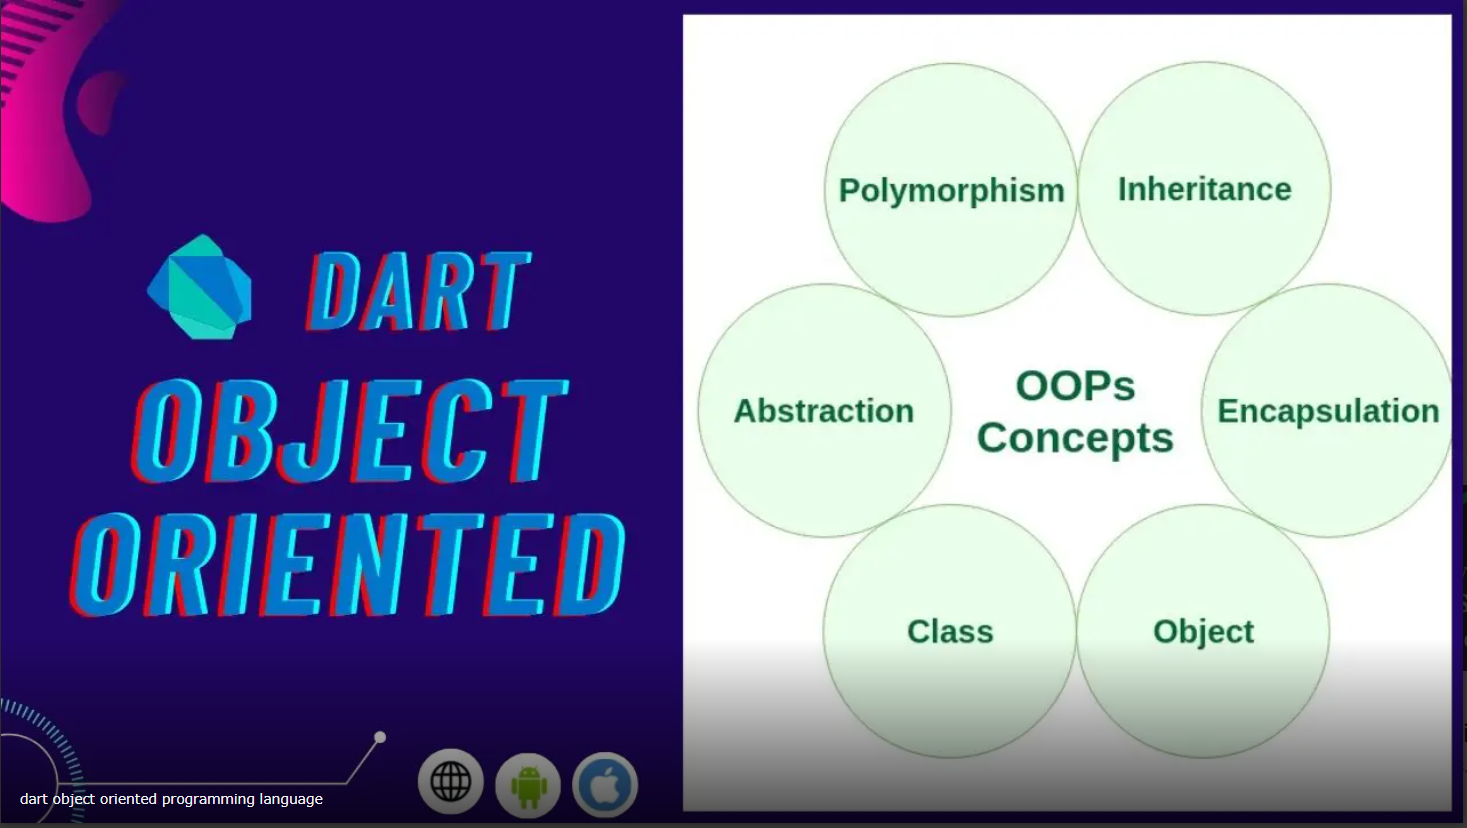
\includegraphics[width=1\textwidth]{Hinhve/oopInDart.png}
    \caption{Các nguyên lý OOP trong Dart}
    \label{fig:oopindart}
\end{figure}

\section{Các đặc trưng hướng đối tượng trong Dart}
\subsection{Đối tượng và lớp}

\begin{itemize}
\item \textbf{Lớp (Class)} là một khuôn mẫu dùng để định nghĩa các thuộc tính và phương thức, các thành phần tĩnh của một kiểu đối tượng. Nó mô tả cấu trúc và hành vi chung của các đối tượng cùng loại.
\item \textbf{Object (Đối tượng)} là thể hiện cụ thể của một lớp, được tạo ra qua constructor của lớp, có trạng thái riêng biệt và có thể thực hiện được các hành vi được định nghĩa trong lớp.
\end{itemize}

Việc sử dụng lớp và đối tượng trong Dart giúp tổ chức dữ liệu và hành vi thành các đơn vị rõ ràng, đóng góp vào tính module hóa của chương trình.

Trong Dart, lớp được khai báo bằng từ khóa \texttt{class}.
\begin{lstlisting}
class class_name {
    // Body of class...
}
\end{lstlisting}

Các đối tượng được khai báo bằng cách sử dụng từ khóa \texttt{new} và theo sau là tên lớp.
\begin{lstlisting}
var object_name = new class_name([ arguments ]);
\end{lstlisting}

Để minh họa cách sử dụng lớp và đối tượng trong Dart, ta xét ví dụ về lớp \texttt{Product} mô phỏng một sản phẩm:

\begin{lstlisting}
class Product {
  // Declare attributes
  String manufacture = '';
  String name = '';
  var price;
  int quantity;

  // Declare constructor
  Product(var price, {int quantity = 0}) {
    this.price = price;
    this.quantity = quantity;
  }

  // Declare methods
  calculateTotal() {
    return this.price * this.quantity;
  }

  showTotal() {
    var total = this.calculateTotal();
    print("The total amount is: $total");
  }
}
\end{lstlisting}

\textbf{Tạo và sử dụng đối tượng:}
\begin{lstlisting}
var product = new Product(600, quantity: 1);
product.showTotal();
product.quantity = 2;
product.showTotal();
\end{lstlisting}

\textbf{Kết quả chạy chương trình:}
\begin{myverbatim}
The total amount is: 600
The total amount is: 1200
\end{myverbatim}

Ở ví dụ trên, lớp \texttt{\textbf{Product}} có các thuộc tính \texttt{manufacture, name, price, quantity}, hàm khơi tạo với 2 tham số: tham số bắt buộc \texttt{price} và tham số tùy chọn \texttt{quantity} với giá trị mặc định là 0. Lớp có hai phương thức \\ \texttt{calculateTotal()} tính tổng giá trị đơn hàng và \texttt{showTotal()} để in ra tổng số tiền.

Trong Dart, từ khóa \textbf{\texttt{this}} dùng để tham chiếu đến chính đối tượng của lớp dùng từ khóa.
Sau đó, khởi tạo đối tượng \texttt{product} từ lớp \textbf{\texttt{Product}} với \texttt{price} là 600 và \texttt{quantity} là 1. Phương thức \texttt{product.showTotal()} tính tổng số tiền dựa trên \texttt{price} và \texttt{quantity}. Tiếp theo, gán lại giá trị cho \texttt{quantity} thành 2 và gọi lại \texttt{showTotal()} để in lại tổng số tiền. 

Trong Dart, một lớp có thể định nghĩa nhiều constructor bằng cách sử dụng \textbf{named constructors}. Điều này cho phép tạo ra các cách khởi tạo đối tượng khác nhau, phục vụ cho các mục đích cụ thể. 

\textit{Ví dụ:}
\begin{lstlisting}
class Student {
  String name;
  int age;

  // Primary constructor
  Student(this.name, this.age);

  // Named constructor for unknown students
  Student.unknown() : name = 'Unknown', age = 0;

  void info() {
    print('Name: $name - Age: $age');
  }
}

void main() {
  var s1 = Student('Ky', 20);
  s1.info(); // Name: Ky - Age: 20

  var s2 = Student.unknown();
  s2.info(); // Name: Unknown - Age: 0
}
\end{lstlisting}

Từ khóa \textbf{static} giúp khai báo các thuộc tính hoặc phương thức không gắn liền với một thể hiện cụ thể, mà thuộc về lớp.

\begin{lstlisting}
class TempConverter {
  static double zeroCelsiusToF = 32;

  static double toCelsius(double fahrenheit) {
    return (fahrenheit - 32) * 5 / 9;
  }
}

void main() {
  print(TempConverter.zeroCelsiusToF); // 32
  print(TempConverter.toCelsius(100)); // 37.777...
}
\end{lstlisting}

Phương thức \texttt{toCelsius()} và thuộc tính \texttt{zeroCelsiusToF}  là static, cho phép gọi trực tiếp qua tên lớp \textbf{\texttt{TempConverter}} mà không cần khởi tạo đối tượng.
\subsection{Đóng gói:} 
Đóng gói là việc gom nhóm dữ liệu và phương thức vào cùng một lớp, hạn chế truy cập bên ngoài nhằm bảo vệ tính toàn vẹn của dữ liệu. Không giống như đa phần các ngôn ngữ khác có các chỉ định truy cập \textbf{public, private, protect}, Dart chỉ thể hiện tính đóng gói thông qua tiền tố \texttt{\_} mà không có giới hạn truy cập một cách tường minh. Đồng thời, Dart hỗ trợ các phương thức getter và setter để kiểm soát việc truy xuất và cập nhật thuộc tính. 

\textit{Ví dụ:}
\begin{lstlisting}
class BankAccount {
  // _balance is a private variable, accessible only within this class
  double _balance;

  BankAccount(this._balance);

  // Getter to access the _balance
  double get balance => _balance;

  // Method to deposit money
  void deposit(double amount) {
    if (amount > 0) {
      _balance += amount;
    }
  }
}
\end{lstlisting}

Ở hàm \texttt{main()}, ta thực hiện thay đổi số dư tài khoản:
\begin{lstlisting}
void main() { 
    var account = BankAccount(1000); 
    account.deposit(500); 
    print(account.balance); // Output: 1500 
}
\end{lstlisting}

Trong ví dụ trên, thuộc tính \texttt{\_balance} được khai báo với tiền tố gạch dưới (\texttt{\_}) cho biết nó là thuộc tính private của lớp \textbf{\texttt{BankAccount}}. Đoạn mã trong hàm \texttt{main()} không thể truy cập trực tiếp \texttt{\_balance}; thay vào đó, ta sử dụng phương thức công khai \texttt{deposit} để thay đổi số dư và \textbf{getter} \texttt{balance} để đọc giá trị. Nhờ vậy, lớp \textbf{\texttt{BankAccount}} kiểm soát được cách thức cập nhật dữ liệu, đảm bảo giá trị \texttt{\_balance} không bị gán giá trị không hợp lệ từ bên ngoài. Đó chính là tính chất đóng gói: nhóm dữ liệu và phương thức xử lý, đồng thời bảo vệ dữ liệu riêng tư.

\subsection{Kế thừa} 
Kế thừa cho phép một lớp con tái sử dụng và mở rộng các thuộc tính và phương thức của lớp cha. Trong Dart, từ khóa \textbf{extends} được sử dụng để kế thừa một lớp khác, và từ khóa \textbf{super} cho phép lớp con truy cập thành phần của lớp cha. Lớp con có thể \textbf{ghi đè (override)} các phương thức của lớp cha bằng chú thích \textbf{\texttt{@override}} để định nghĩa hành vi riêng. Dart chỉ hỗ trợ kế thừa đơn (một lớp con chỉ có một lớp cha) nhưng cho phép sử dụng \textbf{mixins} để mô phỏng đa kế thừa. 

Cú pháp để một lớp con kế thừa một lớp cha:
\begin{lstlisting}
class ChildClass extends ParentClass {
    // Childclass members
}
\end{lstlisting}

Ví dụ về sử dụng từ khóa \textbf{extends}: 
\begin{lstlisting}
// Create a parent class
class Animal {
  String name;
  Animal(this.name);

  void makeSound() {
    print("The animal makes a sound");
  }
}

// Create a child class that inherits using the 'extends' keyword
class Dog extends Animal {
  String breed;

  Dog(String name, this.breed) : super(name);

  @override
  void makeSound() {
    print("The dog barks");
  }
}

void main() {
  // Create an instance of the child class
  var myDog = Dog("Buddy", "Golden Retriever");

  print(myDog.name);       // Output: Buddy
  print(myDog.breed);      // Output: Golden Retriever
  myDog.makeSound();       // Output: The dog barks
}
\end{lstlisting}

Lớp \textbf{\texttt{Animal}} có thuộc tính \texttt{breed}, phương thức \texttt{makeSound()}. Lớp \textbf{\texttt{Dog}} kế thừa từ lớp \textbf{\texttt{Animal}} chỉ ra rằng lớp này kế thừa mọi thành viên từ \textbf{\texttt{Animal}}. Trong lớp con có sử dụng chú thích \texttt{@override} để ghi đè phương thức \texttt{makeSound()} của lớp cha. Ở \texttt{main()}, ta khởi tạo đối tượng \texttt{myDog} thuộc lớp \textbf{\texttt{Dog}} với hai thuộc tính \texttt{name}, \texttt{breed}. Khi thực hiện \texttt{myDog.makeSound()} thì chương trình sẽ thực hiện phương thức \texttt{makeSound()} của lớp con.

Toán tử \textbf{\texttt{cascade (..)}} của Dart cho phép thực hiện liên tiếp nhiều thao tác trên cùng một đối tượng mà không cần lặp lại tên đối tượng. Ví dụ, nếu không dùng \textbf{\texttt{cascade}}, ta phải viết:
\begin{lstlisting}
var paint = Paint();
paint.color = Colors.black;
paint.strokeWidth = 5.0;
\end{lstlisting}

Còn khi sử dụng toán tử \textbf{\texttt{cascade}}, ta chỉ cần:
\begin{lstlisting}
var paint = Paint()
  ..color = Colors.black
  ..strokeWidth = 5.0;
\end{lstlisting}

Nếu đối tượng có thể là null, ta nên dùng toán tử chuỗi null \texttt{(?..)} để tránh lỗi khi gọi phương thức trên null.

\textbf{Giao diện (Interface):} 

Khi một lớp được coi là giao diện thì lớp triển khai của nó phải định nghĩa lại mọi phương thức, thuộc tính có trong giao diện. Để một lớp thực thi giao diện này mà không kế thừa trực tiếp, ta dùng từ khóa 
\textbf{\texttt{implement}} 

\textit{Ví dụ:}
\begin{lstlisting}
class PrinterInterface {
  void display(String text);
}
class ConsolePrinter implements PrinterInterface {
  @override
  void display(String text) {
    print('Printed: $text');
  }
}
void main() {
  PrinterInterface p = ConsolePrinter();
  p.display('Hello Dart'); // Printed: Hello Dart
}
\end{lstlisting}

Lớp \textbf{\texttt{PrinterInterface}} có định nghĩa phương thức \texttt{display()}. Lớp \textbf{\texttt{ConsolePrinter}} được khai báo implements \textbf{\texttt{PrinterInterface}} và cung cấp phần triển khai của \texttt{display()}. Khi chạy, ta thấy in ra \texttt{Printed: Hello Dart}. Sử dụng \texttt{implements} buộc lớp con phải thực thi (override) tất cả các phương thức của interface đã khai báo.
Một lớp có thể thực thi nhiều giao diện cùng một lúc, ví dụ:
\begin{lstlisting}
class Multi implements InterfaceA, InterfaceB {
    ...
}
\end{lstlisting}

\textbf{Mixin:} 

\textbf{Mixin} là một cơ chế tái sử dụng mã cho nhiều lớp khác nhau thông qua từ khóa \texttt{with}. Mixin không được sử dụng trực tiếp để tạo ra một đối tượng, mà nó chứa các phương thức, thuộc tính dùng để gộp vào một lớp khác. 

\textit{Ví dụ:}
\begin{lstlisting}
mixin Flyer {
  void fly() {
    print('Flying');
  }
}
class Bird with Flyer {
  void sing() {
    print('Singing');
  }
}
void main() {
  var b = Bird();
  b.fly();  // Output: Flying
  b.sing(); // Output: Singing
}
\end{lstlisting}

\textbf{\texttt{Flyer}} là một mixin định nghĩa phương thức \texttt{fly()}. Lớp \textbf{\texttt{Bird}} sử dụng \texttt{with Flyer} nên tự động có cả phương thức \texttt{fly()}. Khi chạy, chương trình in Flying và Singing. Như vậy, với mixin ta có thể bổ sung hành vi cho lớp mà không cần thiết lập quan hệ kế thừa.

\subsection{Trừu tượng hóa:} 
Trừu tượng (abstraction) trong OOP cho phép định nghĩa các lớp hoặc phương thức chưa triển khai chi tiết để tạo nên một khái niệm chung. Trong Dart, từ khóa \texttt{abstract} được dùng khai báo một lớp hoặc phương thức là trừu tượng. Một \textbf{lớp trừu tượng} không thể được tạo đối tượng trực tiếp và có thể chứa các phương thức trừu tượng (chỉ khai báo chữ ký, không có phần thân). Các lớp con phải ghi đè và triển khai các phương thức trừu tượng đó. 

\textit{Ví dụ:}
\begin{lstlisting}
abstract class Shape {
  // Abstract method without implementation
  double area();
}

class Square implements Shape {
  double side;
  Square(this.side);

  @override
  double area() {
    return side * side;
  }
}

void main() {
  Shape s = Square(5);
  print('Area of the square: ${s.area()}');
  // Output: Area of the square: 25
}
\end{lstlisting}

Trong ví dụ trên, \textbf{\texttt{Shape}} là lớp trừu tượng khai báo phương thức \texttt{area()} mà không cung cấp định nghĩa. Lớp \texttt{Square} dùng từ khóa \texttt{implements} để triển khai giao diện của \texttt{Shape}, do đó nó phải cung cấp hiện thực cho phương thức \texttt{area()}. Chú thích \texttt{@override} khẳng định rằng \texttt{Square.area()} ghi đè và định nghĩa chức năng cụ thể. Khi trong \texttt{main()}, ta có thể khai báo biến \texttt{s} kiểu \texttt{Shape} nhưng khởi tạo dưới dạng \texttt{Square(5)} để thể hiện rằng \texttt{Square} là một hiện thực của khái niệm trừu tượng \texttt{Shape}. Việc sử dụng lớp trừu tượng cho phép tách biệt phần khai báo chung của các đối tượng cùng loại với phần triển khai cụ thể.

\subsection{Đa hình} 
Đa hình (polymorphism) là một nguyên lý cốt lõi trong lập trình hướng đối tượng, cho phép các đối tượng thuộc các lớp khác nhau được xử lý thông qua một giao diện chung. Nói cách khác, nhiều đối tượng khác loại có thể thực hiện cùng một lời gọi phương thức theo cách riêng của chúng. Trong Dart, đa hình được thực hiện chủ yếu thông qua cơ chế \textbf{kế thừa} và \textbf{ghi đè} phương thức (method overriding). Dart sẽ xác định và thực thi phương thức phù hợp với lớp thực tế của đối tượng tại thời điểm chạy chương trình, giúp mã nguồn linh hoạt và dễ mở rộng hơn.

Ví dụ:
\begin{lstlisting}
class Animal{
    void speak(){
        print('...');
    }
}
class Dog extends Animal{
    @override void speak() { 
        print('Grhh grhh!'); 
    }
}
class Cat extends Animal{
    @override void speak(){
        print("Meo meo!");
    }
}
void main(){
    List<Animal> zoo = [Dog(), Cat()];
    for (var a in zoo)  a.speak(); 
}
\end{lstlisting}

Kết quả chương trình trên in ra là:
\begin{lstlisting}
Grhh grhh!
Meo meo!
\end{lstlisting}

Đoạn mã trên thể hiện tính đa hình khi ta tạo một danh sách \texttt{zoo} chứa các đối tượng thuộc lớp \textbf{\texttt{Dog}} và \textbf{\texttt{Cat}}, cả hai đều là các lớp con của \textbf{\texttt{Animal}}. Mặc dù danh sách khai báo kiểu chung là \textbf{\texttt{Animal}}, khi lặp qua từng phần tử và gọi \texttt{a.speak()}, đối tượng thực thi phương thức tương ứng với lớp của nó: \textbf{\texttt{Dog}} in ra \emph{{}"Grhh grhh!"} còn \textbf{\texttt{Cat}} in ra \emph{{}"Meo meo!"}. Như vậy, cùng một lời gọi \texttt{speak()} nhưng kết quả lại khác nhau tùy vào lớp thực thể, đúng với khái niệm đa hình. 

Đa hình giúp viết mã tổng quát hơn: Người dùng có thể xử lý tập hợp các đối tượng khác nhau cùng họ (kế thừa từ một lớp cha hoặc cùng triển khai một giao diện) mà không cần biết chính xác loại con của chúng, tạo điều kiện thuận lợi cho mở rộng và bảo trì.

\section{Callable class}
Trong Dart, phương thức đặc biệt \verb|call()| cho phép đối tượng của một lớp hoạt động như một hàm. Khi một lớp định nghĩa một phương thức có tên \verb|call|, ta có thể gọi một instance của lớp đó giống như gọi một hàm bình thường, có thể nhận đối số và trả về kết quả. Cú pháp này giúp mở rộng khả năng của lớp, cho phép sử dụng đối tượng như một hàm có thể gọi được (callable). 

\textit{Ví dụ:}
\begin{lstlisting}
class Employee{
    String name;
    Employee(this.name);
    void call() { 
        print('Hello, I am $name'); 
    }
}
void main(){
    var emp = Employee('Alice');
    emp(); //  method call() 
}
\end{lstlisting}

Trong ví dụ trên, khi gọi \verb|emp()|, Dart thực chất sẽ gọi phương thức \verb|call()| của đối tượng \verb|emp|. Vì vậy chương trình sẽ in ra kết quả:
\begin{myverbatim}
    Hello, I am Alice
\end{myverbatim}

\section{Giới thiệu về Async Programming}
\textbf{Lập trình đồng bộ (synchronous)} và \textbf{lập trình bất đồng bộ (asynchronous)} là hai mô hình thực thi khác nhau trong Dart.
\subsection{Lập trình đồng bộ}
Code chạy trong Dart là chạy trên một luồng (thread), dòng code được thi hành hết câu lệnh này sang câu lệnh khác. Nếu một khối lệnh nào đó gây block thread (làm tắc thread) thì toàn bộ ứng dụng sẽ bị treo. 

\textit{Ví dụ:}

\begin{lstlisting} 
const info = "#4fs358w";
getInformation(){
    return info;
}
showInfomation() { 
    var data = getInformation();
    print('Data -' + DateTime.now().toString());
    print(data);
} 
secondFunction(){
    print(Time - ' + DateTime.now().toString());
}
void main() { 
    showInfomation(); 
    secondFunction();
} 
\end{lstlisting}

Giả sử code ở trên nếu \verb|showInformation()| hoặc \verb|getInformation()| mất nhiều thời gian để hoàn thành thì khối lệnh khác như \verb|secondFunction()| phải chờ nó hoàn thành thì mới được thi hành.
\subsection{Lập trình bất đồng bộ}
\textbf{Lập trình bất đồng bộ - Asynchronous}: Khi một phương thức đang thực hiện công việc của mình thì khối lệnh khác - hàm khác vẫn được thi hành. Cơ chế bất đồng bộ là chương trình cho phép phân nhánh quá
trình code hoạt động, làm cho có cảm giác như đa luồng (có thể
vẫn là 1 thread) - có lúc thì chạy code ở nhánh này, có lúc thì
chạy code ở nhánh khác - cảm giác thi hành nhiều việc đồng thời. \\
Dart sử dụng lớp \textbf{\texttt{Future}} với các từ khóa \texttt{async}, \texttt{await}.  

\textbf{Future<T>}: Đối tượng \textbf{\texttt{Future<T>}} trong Dart đại diện cho một giá trị sẽ được cung cấp vào một lúc nào đó trong tương lai (có thể thành công hoặc lỗi). Nó được sử dụng để đánh dấu một phương thức với một kết quả trả về trong tương lai; nghĩa là phương thức trả về đối tượng \textbf{\texttt{Future<T>}} sẽ không có giá trị kết quả thích hợp ngay lập tức mà phải sau một số tính toán tại thời điểm sau đó mới trả về kết quả. 
\begin{lstlisting}
Future<String> fetchData() async {
    await Future.delayed(Duration(seconds: 2));
    return "Get data successfully";
}
\end{lstlisting}

Trong ví dụ trên, \verb|fetchData()| trả về một {\texttt{Future<String>}}, nghĩa là nó sẽ trả về một chuỗi sau khi tác vụ (giả lập bằng \texttt{Future.delayed}) hoàn thành. 

\textbf{Hàm bất đồng bộ async:} Khai báo có từ khóa async phía sau, trả về đối tượng là \textbf{\texttt{Future<T>}}.

Cú pháp: Đặt \texttt{async} trước khối mã của hàm. 

\textit{Ví dụ:}
\begin{lstlisting}
Future<int> functionName() async {
    return 1;
}
\end{lstlisting}

Nếu hàm đó đã khai báo là bất đồng bộ \texttt{async} thì trong hàm có
thể sử dụng cú pháp \texttt{await biểu\_thức}. Khi gặp \texttt{await}, chương trình sẽ tạm dừng thực thi hàm hiện tại và chuyển sang thực thi các tác vụ khác trong hàng đợi sự kiện (event loop). Khi Future hoàn thành, chương trình sẽ tiếp tục thực thi từ dòng mã ngay sau \texttt{await}

\textit{Ví dụ:}
\begin{lstlisting}
Future<String> getInfomation() async {  
    return "Employee information (from Future)"; 
}
Future<void> showInfomation() async { 
    print(await getInfomation()); 
}
void main() { 
    showInfomation(); 
}
\end{lstlisting}

Hàm \verb|getInfomation| được đánh dấu \verb|async| và trả về \verb|Future<String>|. Điều này nghĩa là hàm này khởi tạo một tác vụ bất đồng bộ và sẽ hoàn thành trong tương lai. Từ khóa \verb|await| trong hàm \verb|showInfomation| được sử dụng để đợi giá trị kết quả từ \verb|getInfomation()|. Cụ thể, khi gọi \verb|await getInfomation()|, chương trình sẽ tạm dừng tại vị trí này trong hàm \verb|showInfomation| cho đến khi \verb|getInfomation| trả về giá trị. Sau đó, kết quả nhận được sẽ được in ra. 

\textbf{Xử lý lỗi trong lập trình bất đồng bộ:}
Trong các hàm bất đồng bộ, có thể sử dụng các khối \texttt{try-catch} để xử lý lỗi từ các \texttt{Future}. Đây là một phần quan trọng để đảm bảo chương trình không bị dừng đột ngột khi gặp lỗi. 

\textit{Ví dụ:}
\begin{lstlisting}
Future<String> fetchUserOrder() async {
    throw Exception("Cannot locate user order");
}
Future<void> main() async {
    try {
        var order = await fetchUserOrder();
        print(order);
    } catch (err) {
        print('Caught error: $err');
    }
}
\end{lstlisting}

Kết quả in ra của chương trình trên là:
\begin{lstlisting}
Caught error: Exception: Cannot locate user order
\end{lstlisting}
\textbf{Streams:} Ngoài Future, Dart còn hỗ trợ \textbf{\texttt{Stream}} để xử lý các chuỗi sự kiện bất đồng bộ, như dữ liệu từ mạng hoặc sự kiện người dùng. \textbf{\texttt{Stream}} đại diện cho một chuỗi các giá trị được phát ra theo thời gian. 

\textit{Ví dụ:}
\begin{lstlisting}
Stream<int> getNumbers() async* {
    for (int i = 0; i < 5; i++) {
        await Future.delayed(Duration(seconds: 1));
        yield i;
    }
}

Future<void> main() async {
    await for (var number in getNumbers()) {
        print(number);
    }
}
\end{lstlisting}

Kết quả in ra của chương trình trên là:
\begin{myverbatim}
0 (sau 1s)
1 (sau 1s)
2 (sau 1s)
3 (sau 1s)
4 (sau 1s)
\end{myverbatim}
\end{document}
